\documentclass[12pt]{article}
\usepackage{amsmath}
\usepackage{hyperref}
\usepackage{graphicx}
\usepackage{fullpage}
\title{A Pita-Form With No Crease}
\author{Alex Cole and Ben Kraft}
\begin{document}
\maketitle

\section{The problem:}
In \textit{Generalized D-Forms Have No Spurious Creases}, Eric Demaine and Gregory Price show that all of the creases in the flat components of a seam form (a convex surface that is flat everywhere except finitely many smooth curves) occur between vertices or are tangent to the seams. As a corallary, this implies that pita-forms (or seam forms made from a sewing a single smooth convex shape along its boundary) must have only 1 crease though the flat region that runs between the 2 vertices (the start and end points of the sewing). Up until now, all examples of pita-forms have exhibited this crease, but at \url{http://gfalop.org/closed.open}, it was asked whether pita-forms always have this crease. Here we demonstrate a pita-form with no crease.

\section{Our construction}
Our surface is created by taking the convex hull of a unit spring of height $h$. So we look at the curve traced by the parametric equation 
$$(x(t), y(t), z(t)) = \left(\cos(t), \sin(t), \frac{ht}{2\pi} \right) \text{ for } t \in [0, 2\pi]$$
and take the convex hull. Letting $h=5$ and approximating the curve with 150 points, we get something that looks like:

\begin{center}
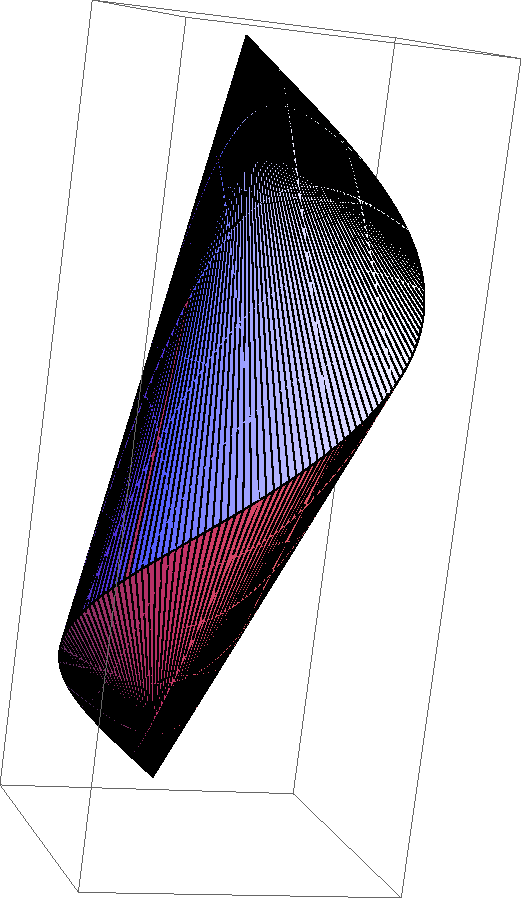
\includegraphics[scale=.6]{pita_h=5_n=150.pdf}
\end{center}

\subsection{Is it a pita form?}
This is a natural first question to ask about the surface. 

First, note that every point of the parametric equation is actually on the surface and furthermore, the segment running from each point of the coil to each of the 2 vertices is on the surface, so the entire surface is ruled and therefore flat. This is fairly clear when you look at the 50 point approximation below:
\begin{center}
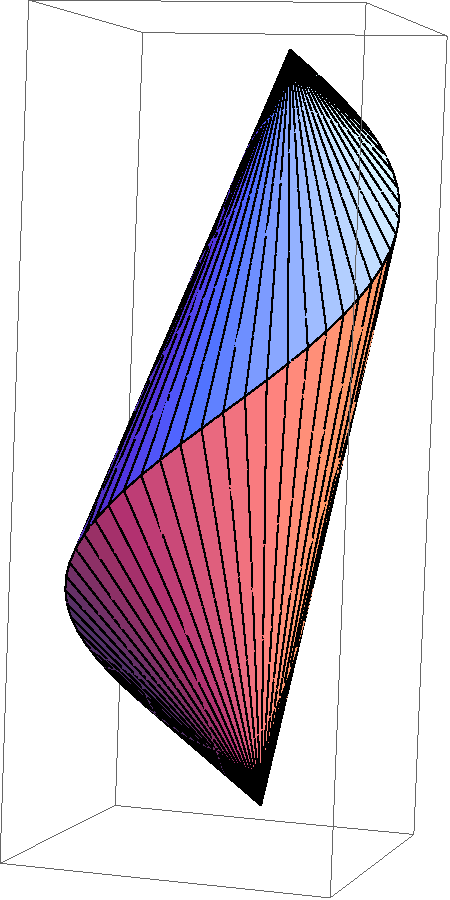
\includegraphics[scale=.6]{pita_h=5_n=50.pdf}
\end{center}

Now to show that it is a pita form, we need to check that it comes from a smooth convex shape. To examine this we can look at 150 point approximations of the unfoldings of it along the edge for $h=3$, 5, and 7:
\begin{center}
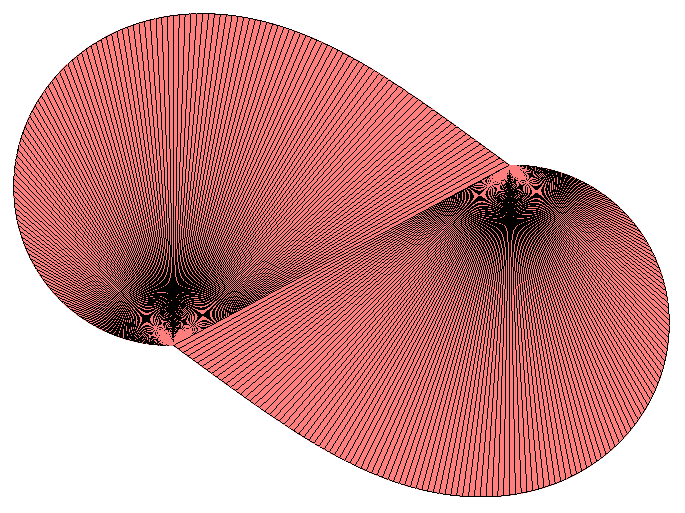
\includegraphics[scale=.4]{unfold_h=3_n=150.pdf}
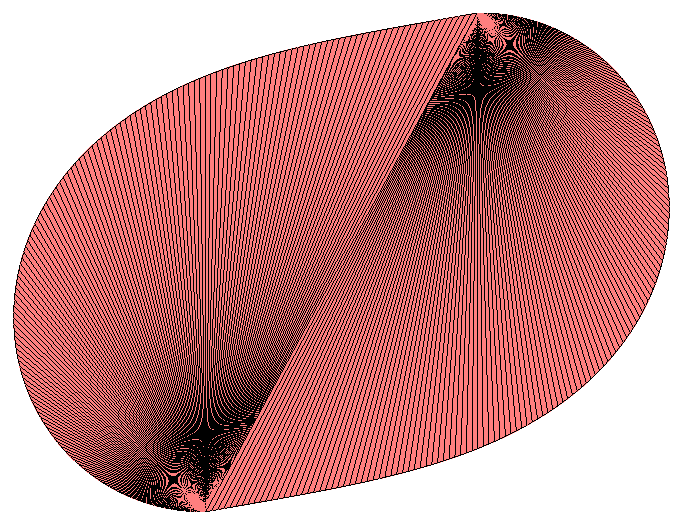
\includegraphics[scale=.4]{unfold_h=5_n=150.pdf}
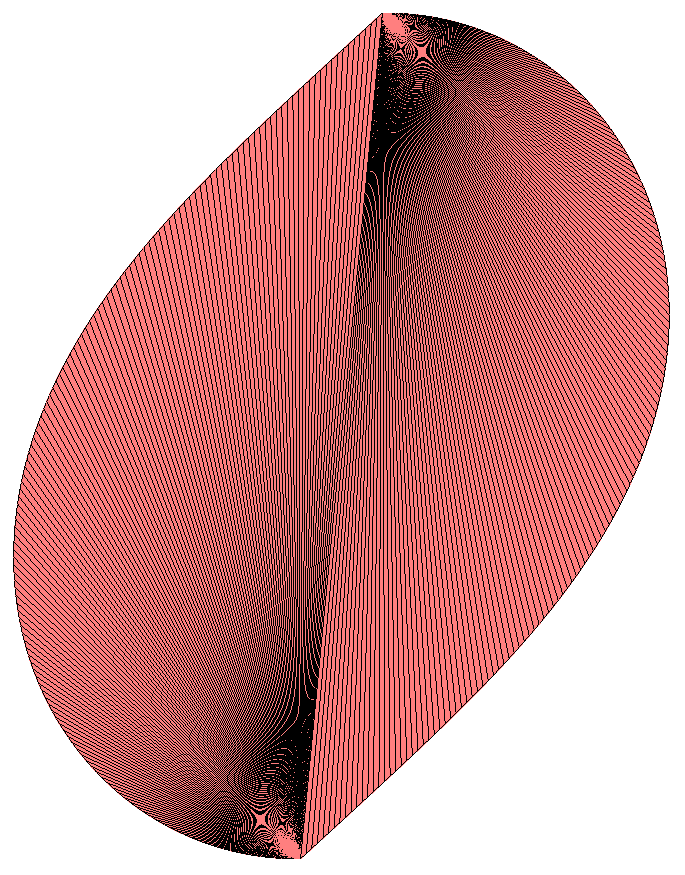
\includegraphics[scale=.4]{unfold_h=7_n=150.pdf}
\end{center}

As you can see, it is clearly smooth and convex aside from the 2 points that form the vertices of the sewed surface. When $h=3$ those points have over $180^\circ$ of material around each of them making the unfolding concave and not smooth. Similarly when $h=7$ there is less than $180^\circ$ of material around each vertex causing the shape to be convex, but still not smooth. But by continuity, there is some $h^*$ in between 3 and 7 such that there is exactly $180^\circ$ of material around each vertex causing the shape to be smooth. We think that $h^*$ is around 5, but we don't know the precise value. So when $h=h*$ our figure is a pita-form.

\subsection{Is there a crease?}
Getting back to our original question, did we actually construct a pita form without a crease?
\begin{center}
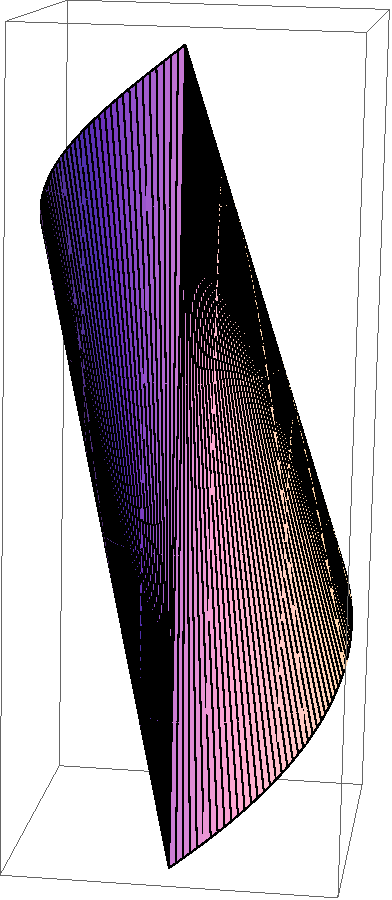
\includegraphics[scale=.6]{crease_h=5_n=150.pdf}
\end{center}
Assume that there is a crease. Then it must be between the 2 vertices of our pita-form. Also if it is a crease, then there is an infinite family of tangent planes tangent to the pita-form along the crease. But our original parametric curve lies along a cylinder of radius 1 along the $z$-axis. So looking at our tangent plane, we see that it must also be tangent to this cylinder and the cylinder is smooth, so there is only 1 tangent plane to each vertical segment on the surface. This means that there is a unique tangent plane to the crease, so it isn't a crease at all. 

This means that this is in fact a pita-form with no crease. Woo hoo!

\end{document}